% easychair.tex,v 3.5 2017/03/15

\documentclass{easychair}
%\documentclass[EPiC]{easychair}
%\documentclass[EPiCempty]{easychair}
%\documentclass[debug]{easychair}
%\documentclass[verbose]{easychair}
%\documentclass[notimes]{easychair}
%\documentclass[withtimes]{easychair}
%\documentclass[a4paper]{easychair}
%\documentclass[letterpaper]{easychair}

\usepackage{doc}
\usepackage{wrapfig}

% use this if you have a long article and want to create an index
% \usepackage{makeidx}

% In order to save space or manage large tables or figures in a
% landcape-like text, you can use the rotating and pdflscape
% packages. Uncomment the desired from the below.
%
% \usepackage{rotating}
% \usepackage{pdflscape}

\usepackage{amsfonts}

\usepackage{tikz}
\usetikzlibrary{automata, positioning, arrows}
\tikzset{
  ->, % makes the edges directed
  >=stealth', % makes the arrow heads bold
  node distance=2.5cm, % specifies the minimum distance between two nodes. Change if necessary.
  every state/.style={thick, fill=gray!10}, % sets the properties for each ’state’ node
  initial text=$ $, % sets the text that appears on the start arrow
}

%% Front Matter
%%
% Regular title as in the article class.
%
\title{Type-safe Bidirectional Channels in Idris 2}

% Authors are joined by \and. Their affiliations are given by \inst, which indexes
% into the list defined using \institute
%
\author{Guillaume Allais\inst{1}}

% Institutes for affiliations are also joined by \and,
\institute{
  University of Strathclyde,
  Glasgow, Scotland, United Kingdom\\
  \email{guillaume.allais@strath.ac.uk}}

%  \authorrunning{} has to be set for the shorter version of the authors' names;
% otherwise a warning will be rendered in the running heads. When processed by
% EasyChair, this command is mandatory: a document without \authorrunning
% will be rejected by EasyChair

\authorrunning{Guillaume Allais}

% \titlerunning{} has to be set to either the main title or its shorter
% version for the running heads. When processed by
% EasyChair, this command is mandatory: a document without \titlerunning
% will be rejected by EasyChair
\titlerunning{Type-safe Bidirectional Channels in Idris 2}

\begin{document}

\maketitle

%------------------------------------------------------------------------------
\subsubsection*{Introduction}

Session types are a kind of channel typing discipline ensuring that the
communication patterns of concurrent programs abide by a shared protocol.

\newcommand{\nat}{\ensuremath{\mathbb{N}}}
\newcommand{\recvar}[1]{\ensuremath{\mathit{x}}}
\newcommand{\send}[2]{\ensuremath{!#1.~#2}}
\newcommand{\recv}[2]{\ensuremath{?#1.~#2}}
\newcommand{\select}[2]{\ensuremath{#1 \mathop{\oplus} #2}}
\newcommand{\offer}[2]{\ensuremath{#1 \mathop{\&} #2}}
\newcommand{\smallest}[2]{\ensuremath{\mu #1.~#2}}
\newcommand{\largest}[2]{\ensuremath{\nu #1.~#2}}
\newcommand{\stopsesh}{\ensuremath{\mathtt{end}}}

Limiting ourselves to two communicating parties, we demonstrate how to give a
type-safe implementation of bidirectional channels typed using protocols closed
under typed sends (\send{A}{\cdot}),
typed receives (\recv{A}{\cdot}),
branch offerings (\offer{\cdot}{\cdot}),
branch selections (\select{\cdot}{\cdot}),
and smallest (\smallest{x}{\cdot})
and largest (\largest{x}{\cdot}) fixpoints.

\[
p,~ q,~ \dots
  \; ::= \; \recvar{x}
  \; | \; \smallest{x}{p}
  \; | \; \largest{x}{p}
  \; | \; \send{A}{p}
  \; | \; \recv{A}{p}
  \; | \; \stopsesh{}
  \; | \; \offer{p}{q}
  \; | \; \select{p}{q}
\]

\noindent
\begin{wrapfigure}{r}{.5\textwidth}
  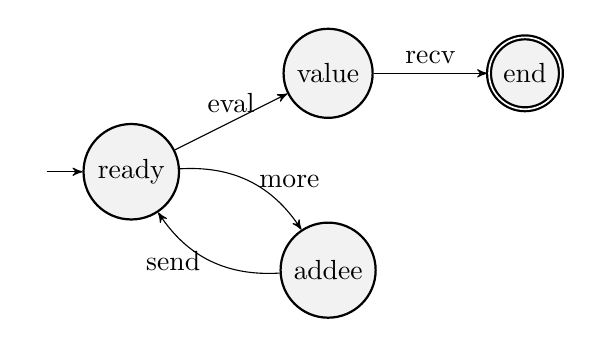
\begin{tikzpicture}
    \node[state, initial]                  (q1)  {ready};
    \node[state, right of=q1, yshift=1.25cm]              (q2r) {value};
    \node[state, below of=q2r]              (q2l) {addee};
    \node[state, accepting, right of=q2r]  (q3)  {end};
    \draw
      (q1) edge[bend left, right] node{more} (q2l)
      (q1) edge[above]             node{eval} (q2r)
      (q2l) edge[bend left, left]   node{send \nat} (q1)
      (q2r) edge[above]             node{recv \nat} (q3);
  \end{tikzpicture}
  \caption{The ``adder'' protocol}
\end{wrapfigure}
The session
$
\largest{x}{(\offer
  {(\overbrace{\recv{\nat}{\recvar{x}}}^{\text{more}})}
  {(\overbrace{\send{\nat}{\stopsesh}}^{\text{eval}})})}
$
types a server for the ``adder'' protocol: it accepts an
arbitrary sequence of natural numbers (sent by repeatedly
selecting the \emph{more} branch) before sending back their
sum as a single number (when the \emph{eval} branch is
ultimately selected) and terminating.

The encoding of the protocol uses a largest fixpoint to
describe the server because the client is the one responsible
for ensuring the process terminates by eventually selecting
the \emph{eval} branhc.

%------------------------------------------------------------------------------
\subsubsection*{Implementation}

The key idea behind this safe implementation is to collect all of the sent
and received types used in a protocol and to manufacture a big sum type
in which we can inject all of these values.
%
Our implementation of this sum type is based on a type safe realisation of
Kiselyov and Sabry's open union type~\cite{DBLP:conf/haskell/KiselyovSS13}
using the encoding of scope-safe
De Bruijn indices~\cite{MANUAL:journals/math/debruijn72}
introduced by Brady in the implementation of
Idris 2~\cite{DBLP:conf/ecoop/Brady21}.
%
This gives us an encoding that has constant time injections and
(potentially failing) projections in and out of the shared sum type.


One challenge comes from the fact that the session type, by design,
changes afer communications.
%
The solution is to record an offset remembering where we currently
are in the protocol and thus allowing us to keep injecting values to
be sent into the initial shared sum type.
%
Our offsets are proven correct using a gadget that can be understood
as a cut down version of McBride's one hole
contexts~\cite{DBLP:conf/popl/McBride08}. Instead
of recording the full path followed by our programs in the finite
state machine describing the protocol, we record a de-looped version
of the path which is sufficient for our purpose.


%------------------------------------------------------------------------------
\subsubsection*{Limitations and Future Work}

\paragraph{Encoding Uniqueness via Linear Types}
Unlike Brady's prior work in Idris 1~\cite{DBLP:journals/aghcs/Brady17},
we are using Idris 2 which does not currently have uniqueness types.
We are forced to use the linearity granted to us by
Quantitative Type Theory (QTT)~\cite{DBLP:conf/birthday/McBride16,DBLP:conf/lics/Atkey18}
to emulate uniquess which adds a degree of noise to the implementation.
We would ideally want a system combining both to benefit from enhanced
expressivity and efficiency as described by Marshall, Vollmer,
and Orchard~\cite{DBLP:conf/esop/MarshallVO22}.

\paragraph{Small Runtime Overhead}
In the most expressive version of our library, we compute a handful
of key offset values by induction over the protocol. Correspondingly
the protocol is not marked as erased anymore and, if compilation does
not specialise the relevant combinators agressively, then we may very
well be evaluating these relatively small computations at runtime.
%
As far as we understand, directly adding typed staging to Idris 2
through the use of a two-level type theory à la
Kov{\'{a}}cs~\cite{DBLP:journals/pacmpl/Kovacs22} would not be
enough to solve our issue: the protocol does need to persist
through staging, but merely move from QTT's unrestricted to its
erased modality.

\paragraph{Ergonomics}
We found writing the types of inner loops of programs with non-trivial
communication patterns to be tedious as they expose quite a lot of the
powerful but noisy encoding of syntaxes with binding we use.




%------------------------------------------------------------------------------
%% BIBLIOGRAPHY

\bibliographystyle{plain}
%\bibliographystyle{alpha}
%\bibliographystyle{unsrt}
%\bibliographystyle{abbrv}
\bibliography{session}

\end{document}
